\documentclass[runningheads,a4paper]{llncs}
\usepackage[T1]{fontenc}
\usepackage{graphicx}
\usepackage{booktabs}
\usepackage{capt-of}
\usepackage{cite}
\usepackage{tikz}
\usetikzlibrary{arrows.meta,positioning}
\usepackage[hidelinks]{hyperref}
\newcommand{\model}[1]{{\hyphenpenalty=10000 \exhyphenpenalty=10000 \textsf{#1}}}

\begin{document}
\title{Medical-LLM Supervision for Peer Retrieval in a Rare-Disease Community}
\titlerunning{Medical-LLM Supervision for Rare-Disease Peer Retrieval}
\author{Max Lübbering\inst{1,4}\fnmsep\thanks{These authors contributed equally to this work.}
    \and Thiago Bell Felix de Oliveira\inst{1}\fnmsep\protect\footnotemark[1]
    \and Corinna Lewis Schmalohr\inst{1,2}
    \and David Berghaus\inst{1,4}
    \and Lorenz Grigull\inst{2}
    \and Rafet Sifa\inst{1,2}
    }
\authorrunning{Max Lübbering and Thiago Bell}
\institute{Fraunhofer IAIS, Germany \and University of Bonn, Germany \and University Hospital Bonn, Germany \and Lamarr Institute, Germany}
\maketitle

\begin{abstract}
People affected by rare diseases seek peers with shared experiences, but
diagnoses are often incomplete and interaction histories too sparse for learning.
On a non-profit peer platform with 3,584 profiles, we use a medical LLM, MedGemma
27B, as relevance judge: it grades 6.3 million profile pairs with an
expert-informed rubric, and students learn these grades so that members,
including newcomers, are matched from a single profile encoding. A three-part
evaluation anchors teacher and students to a healthcare professional, to
historical user ratings and to each other. The LLM agrees more closely with the
professional than a pre-existing rule-based recommender (Spearman 0.78 versus 0.53), and its
students agree as closely. For held-out newcomer users, a fine-tuned embedding
retrieval model orders their rated peers better than the rules (NDCG@5 0.77 versus
0.69) and slightly better than the LLM itself; once a new profile is transcribed, it
ranks a new member against the other 3,583 profiles in 8\,ms instead of 1.7\,h on
one A100 GPU. It concentrates suggestions less than pairwise multilayer perceptron (MLP) scorers but more
than the rules, so deployment should monitor exposure. A theory of change links
these results to helpful peer contact and defines the outcome study that tests it.
\keywords{Peer recommendation \and Rare diseases \and Online health communities
\and LLM relevance judgments \and Knowledge distillation}
\end{abstract}

\section{Introduction}\label{sec:intro}
Rare diseases collectively affect an estimated 263--446 million people
worldwide~\cite{nguengang2020estimating}, with individual communities
widely dispersed~\cite{titgemeyer2022facebook}.
Reaching a diagnosis can itself take years: a European survey of 6,507 respondents reported a mean of 4.7 years (median 0.8) from symptom onset to confirmed diagnosis~\cite{faye2024time}.
Online communities offer practical knowledge and emotional
support~\cite{doyle2024support}, but members must still find someone with
whom an exchange would be useful.

Matching on recorded diagnoses alone can miss comparable experiences,
particularly when a diagnosis is missing or provisional. Symptoms and
caregiving experiences may also matter.

We study a non-profit platform for patients, relatives and healthcare
professionals (HCPs). Its current recommender, which we will call \emph{deployed rules}, is a
hand-written rule system that scores a pair from structured profile fields and
disease-ontology relationships~\cite{fendrich2026development,berger2024tackling}. User ratings offer an alternative
training signal, but cover few possible pairs and are absent for new members.
Our approach instead asks a medical large language model (LLM) about potential
conversational benefit. MedGemma 27B~\cite{sellergren2025medgemma}, an open medical LLM that is competitive
with open models of similar size on medical benchmarks and runs locally, is the \emph{teacher};
since scoring every candidate with it would take thousands of
long generations per query, smaller \emph{student} matchers, an embedding retrieval model and a
pairwise multilayer perceptron (MLP), learn its grades
and match new members from their profile alone (Fig.~\ref{fig:pipeline}).

\begin{figure}[!htb]
\centering
\definecolor{plPanel}{HTML}{DAE8FC}\definecolor{plPanelLine}{HTML}{6C8EBF}%
\definecolor{plCard}{HTML}{FFE6CC}\definecolor{plCardLine}{HTML}{D79B00}%
\definecolor{plDoc}{HTML}{FFF2CC}\definecolor{plDocLine}{HTML}{D6B656}%
\definecolor{plScore}{HTML}{F8CECC}\definecolor{plScoreLine}{HTML}{B85450}%
\definecolor{plGrey}{HTML}{666666}\definecolor{plBadge}{HTML}{34425A}%
\begin{tikzpicture}[
  x=1cm, y=1cm,
  every node/.style={font=\fontfamily{phv}\fontsize{5.9}{7.0}\selectfont,
    inner sep=0pt, align=center, text=black},
  panel/.style={draw=plPanelLine!50, fill=plPanel, rounded corners=8pt, line width=0.5pt},
  ptitle/.style={font=\fontfamily{phv}\fontsize{6.8}{7.9}\selectfont\bfseries},
  card/.style={draw=plCardLine, fill=plCard, rounded corners=4.5pt, line width=0.5pt},
  flow/.style={-{Stealth[length=1.3mm, width=1.1mm]}, line width=0.6pt},
  sheet/.style={font=\fontfamily{phv}\fontsize{5.4}{6.3}\selectfont},
  badge/.style={circle, fill=plBadge, text=white, minimum size=0.26cm,
    font=\fontfamily{phv}\fontsize{4.9}{4.9}\selectfont\bfseries},
]
\useasboundingbox (0,0) rectangle (12.18,4.05);
\newcommand{\plDocShape}[4]{%
  \filldraw[draw=plDocLine, fill=plDoc, line width=0.45pt]
    (#1,#2) -- ++(#3,0) -- ++(0,#4-0.14) -- ++(-0.14,0.14) -- ++(-#3+0.14,0) -- cycle;
  \draw[plDocLine, line width=0.45pt] (#1+#3-0.14,#2+#4) -- ++(0,-0.14) -- ++(0.14,0);}
\newcommand{\plStack}[4]{%
  \plDocShape{#1-#3/2+0.12}{#2-#4/2+0.12}{#3}{#4}%
  \plDocShape{#1-#3/2+0.06}{#2-#4/2+0.06}{#3}{#4}%
  \plDocShape{#1-#3/2}{#2-#4/2}{#3}{#4}}
\newcommand{\plWave}[6]{%
  \filldraw[draw=#6, fill=#5, line width=0.5pt]
    (#1,#2+0.07) -- (#1,#2+#4) -- (#1+#3,#2+#4) -- (#1+#3,#2+0.07)
    .. controls (#1+0.7*#3,#2+0.2) and (#1+0.45*#3,#2-0.1) .. (#1+0.2*#3,#2+0.01)
    .. controls (#1+0.1*#3,#2+0.04) .. cycle;}
\newcommand{\plNet}[3]{%
  \begin{scope}[shift={(#1,#2)}, x=#3cm, y=#3cm]
    \draw[plCardLine, line width=0.65pt] (90:1) -- (30:1) -- (-30:1) -- (-90:1) -- (-150:1) -- (150:1) -- cycle;
    \foreach \a in {(-0.25,0.5),(0.25,0.5)}
      \foreach \b in {(-0.45,0),(0,0),(0.45,0)} \draw[plCardLine, line width=0.35pt] \a -- \b;
    \foreach \b in {(-0.45,0),(0,0),(0.45,0)}
      \foreach \c in {(-0.25,-0.5),(0.25,-0.5)} \draw[plCardLine, line width=0.35pt] \b -- \c;
    \foreach \p in {(-0.25,0.5),(0.25,0.5),(-0.45,0),(0,0),(0.45,0),(-0.25,-0.5),(0.25,-0.5)}
      \filldraw[draw=plCardLine, fill=plCard, line width=0.4pt] \p circle (0.12);
  \end{scope}}
\newcommand{\plPerson}[3]{%
  \begin{scope}[shift={(#1,#2)}, x=#3cm, y=#3cm, line width=0.5pt, plGrey]
    \draw (0,0.55) -- (0,1.05); \draw (-0.26,0) -- (0,0.55) -- (0.26,0);
    \draw (-0.32,0.88) -- (0.32,0.88); \filldraw[fill=white] (0,1.25) circle (0.2);
  \end{scope}}
\newcommand{\plConvert}[2]{%
  \begin{scope}[shift={(#1,#2)}, line width=0.5pt, plGrey]
    \draw[fill=white, rounded corners=0.6pt] (-0.40,-0.17) rectangle (-0.12,0.17);
    \node[text=plGrey, font=\fontfamily{phv}\fontsize{5}{5}\selectfont\bfseries] at (-0.26,0) {\{\,\}};
    \draw[fill=white, rounded corners=0.6pt] (0.12,-0.17) rectangle (0.40,0.17);
    \node[text=plGrey, font=\fontfamily{phv}\fontsize{5.6}{5.6}\selectfont\bfseries] at (0.26,0) {\#};
    \draw[-{Stealth[length=0.9mm, width=0.9mm]}] (-0.08,0) -- (0.08,0);
  \end{scope}}
\newcommand{\plRules}[2]{%
  \begin{scope}[shift={(#1,#2)}, line width=0.45pt, plGrey]
    \draw[fill=white, rounded corners=0.8pt] (-0.17,-0.2) rectangle (0.17,0.2);
    \foreach \y in {0.1,0,-0.1} {\draw (-0.11,\y-0.03) rectangle ++(0.06,0.06);
      \draw (-0.01,\y) -- (0.11,\y);}
  \end{scope}}

\filldraw[panel] (1.10,0) rectangle (4.55,4.05);
\filldraw[panel] (4.65,0) rectangle (8.52,4.05);
\filldraw[panel] (8.62,0) rectangle (12.18,4.05);
\node[ptitle] at (2.825,3.69) {(1) Source pseudonymized\\profile data};
\node[ptitle] at (6.585,3.69) {(2) Collect LLM-sourced\\teacher grades};
\node[ptitle] at (10.40,3.69) {(3) Derive light-weight\\matchers};

\plStack{0.46}{1.72}{0.92}{1.12}
\node[sheet] at (0.46,1.64) {\textbf{3,584}\\JSON\\profiles};

\filldraw[card] (1.22,1.86) rectangle (2.88,3.30);
\node[anchor=north] at (2.05,3.17) {\textbf{Collect} human\\judgments};
\plPerson{1.70}{1.98}{0.26}\plPerson{2.05}{2.11}{0.26}\plPerson{2.40}{1.98}{0.26}
\plWave{3.04}{2.63}{1.44}{0.67}{plScore}{plScoreLine}
\node[sheet, anchor=north] at (3.76,3.20) {\textbf{HCP scores}\\66 pairs};
\plWave{3.04}{1.86}{1.44}{0.67}{plScore}{plScoreLine}
\node[sheet, anchor=north] at (3.76,2.43) {\textbf{User ratings}\\$\approx$15k records};
\node[badge] at (4.44,3.30) {E1};
\node[badge] at (4.44,2.53) {E2};

\filldraw[card] (1.22,0.14) rectangle (2.88,1.58);
\node[anchor=north] at (2.05,1.45) {\textbf{Translate} and\\\textbf{transcribe}};
\node[sheet] at (2.05,0.80) {DE $\rightarrow$ EN\\with a local LLM};
\plConvert{2.05}{0.40}
\plStack{3.73}{0.80}{1.14}{1.08}
\node[sheet] at (3.73,0.74) {\textbf{Markdown}\\profile\\texts};

\draw[flow] (1.03,1.72) -- (1.08,1.72) |- (1.22,2.58);
\draw[flow] (1.08,1.72) |- (1.22,0.86);
\draw[flow] (2.88,2.99) -- (3.04,2.99);
\draw[flow] (2.88,2.22) -- (3.04,2.22);
\draw[flow] (2.88,0.86) -- (3.16,0.86);
\node[sheet, text=plGrey, align=center] at (0.50,0.52) {+\,ontology\\context};
\draw[flow, plGrey] (0.90,0.52) -- (1.22,0.52);

\plWave{4.77}{1.98}{1.85}{1.32}{plDoc}{plDocLine}
\node[sheet, align=left, anchor=north west] at (4.88,3.19)
  {\textbf{Matching prompt}\\0--5 rubric: +1 if \ldots\\Profiles A, B: \ldots\\Score:};
\filldraw[card] (4.77,0.14) rectangle (6.62,1.62);
\node[anchor=north] at (5.695,1.49) {\textbf{Grade} pairs with\\LLM-as-a-judge};
\node[sheet] at (5.695,0.86) {MedGemma 27B};
\plNet{5.695}{0.42}{0.21}
\draw[flow] (5.695,2.04) -- (5.695,1.62);
\draw[flow] (4.42,0.86) -- (4.77,0.86);

\plWave{6.80}{1.10}{1.62}{1.64}{plScore}{plScoreLine}
\node[sheet, align=left, anchor=north west] at (6.91,2.64)
  {\textbf{Teacher grades}\\{\color{plGrey}$\approx$6M pairs, 0--5}\\Profile 7 $\times$ 9:\enspace 2\\Profile 9 $\times$ 6:\enspace 1\\\ldots\\Profile 4 $\times$ 5:\enspace 5};
\draw[flow] (6.62,0.86) -| (7.30,1.13);

\draw[plGrey!80, line width=1pt] (10.66,0.20) -- (10.66,3.24);
\filldraw[card] (8.72,1.86) rectangle (10.57,3.30);
\node[anchor=north] at (9.645,3.17) {\textbf{Fine-tune}\\embedding\\retrieval model};
\plNet{9.645}{2.12}{0.19}
\filldraw[card] (8.72,0.14) rectangle (10.57,1.58);
\node[anchor=north] at (9.645,1.45) {\textbf{Train} pairwise\\MLP scorer on\\profile vectors};
\plNet{9.645}{0.40}{0.19}
\node[badge] at (8.955,1.72) {E3};
\node[sheet, anchor=west] at (9.135,1.72) {held-out fidelity};

\filldraw[card] (10.75,1.86) rectangle (12.08,3.30);
\node[anchor=north] at (11.415,3.17) {\textbf{Apply}\\pretrained\\encoders};
\plNet{11.415}{2.12}{0.19}
\filldraw[card] (10.75,0.14) rectangle (12.08,1.58);
\node[anchor=north] at (11.415,1.45) {\textbf{Apply}\\deployed\\rules};
\plRules{11.415}{0.40}

\draw[flow] (8.42,1.91) -- (8.575,1.91) |- (8.72,2.58);
\draw[flow] (8.575,1.91) |- (8.72,0.86);
\end{tikzpicture}
\Description{Three blue stage panels, redrawn from the original overview. Stage 1: 3,584 pseudonymized JSON profiles feed two tasks: collecting human judgments, which yields scores from one HCP on 66 pairs (E1) and about 15,000 user rating records (E2), and LLM translation from German to English and transcription into Markdown profile texts, with disease-ontology context added before transcription. Stage 2: a matching prompt with a 0 to 5 rubric and the profile texts are graded by MedGemma 27B as an LLM judge, yielding teacher grades for about 6 million of the 6.4 million attempted pairs. Stage 3: the teacher grades train two students, a fine-tuned embedding retrieval model and a pairwise MLP scorer on frozen profile vectors, whose held-out fidelity is E3; pretrained embedding retrieval models and the deployed rules serve as baselines.}
\caption{Pipeline overview (MLP: multilayer perceptron). Teacher grades are the
only student supervision; students encode the same Markdown texts. HCP scores
(E1; pairs sampled across teacher grades) and user ratings (E2) evaluate teacher
and students; E3 measures the students' fidelity to the teacher on users excluded
from training (Sect.~\ref{sec:findings}). Example rows are placeholders.}
\label{fig:pipeline}
\end{figure}


We bring LLM relevance judging and distillation (Sect.~\ref{sec:related}) to peer
discovery through medical and lived experience.
We ask whether the teacher agrees with an expert (E1), aligns with user ratings
(E2), and transfers its ordering to students (E3). Separating these questions
responds to LLM-judgment concerns~\cite{faggioli2023perspectives,dietz2025judges}.
Our contributions are (i) a three-part evaluation that anchors an LLM teacher
and its students to an expert and to user ratings, with exact chance levels;
(ii) evidence that a fine-tuned embedding retrieval model is as faithful to the teacher and as
close to the expert as pairwise MLP scorers, beats the deployed rules on newcomers'
ratings, and spreads exposure more evenly; (iii) an exposure
audit showing that students concentrate suggestions beyond what their labels
imply; and (iv) a testable theory of change.

\section{Related Work}
\label{sec:related}
\paragraph{LLMs as Relevance Judges.}
Prompted LLMs can label relevance as accurately as human labellers and have been
deployed for large-scale labelling~\cite{thomas2024preferences}; an open-source
toolkit reproduces these results~\cite{upadhyay2024umbrela}. Others caution that
such labels need human validation~\cite{faggioli2023perspectives,dietz2025judges}
and that evaluating systems with labels from the model that trained them is
circular~\cite{dietz2025judges,soboroff2025judgments};
stratified sampling by the LLM's label reduces the human effort for this
validation~\cite{merlo2026stratified}. We follow this advice: the teacher is
anchored to an expert (E1) and to member ratings (E2), and agreement with the
teacher (E3) is reported as fidelity, not as quality.

\paragraph{Synthetic Labels and Distillation for Retrieval.}
LLMs generate training queries for
rerankers~\cite{bonifacio2022inpars} and retrievers~\cite{dai2023promptagator}, their rankings can be
distilled into smaller rerankers~\cite{sun2023rankgpt}, and their graded relevance
scores can train dense encoders directly~\cite{bixse2025}; knowledge distillation
also transfers a slow ranker's score margins to efficient
students~\cite{hofstatter2020distillation}. These methods rank documents for
queries. We instead grade pairs of members of one community with an
expert-informed rubric and distill the grades into one vector per profile with a
ranking loss over graded labels~\cite{huang2024cosent}, so that newcomers need
neither interactions nor teacher calls.

\paragraph{Peer and People Recommendation.}
In a small cancer peer-mentoring study, participants rated sample posts as the most
helpful profile element for deciding whether to contact a mentor~\cite{hartzler2016peer}; a later field study examined recommendations
through connection behavior~\cite{levonian2025peer}. Peer discovery is a social
task, distinct from matching clinical cases for gene discovery, as in Matchmaker
Exchange~\cite{philippakis2015matchmaker}. Earlier platform studies explored LLM
profile augmentation~\cite{berger2024tackling} and feedback-trained
matchers~\cite{berger2024advancing,berger2024optimizing}. Here, synthetic grades
train students and ratings serve only for evaluation, so results are not directly
comparable. People recommenders are often reciprocal: a match succeeds only if both
sides accept it, so recommenders combine both users'
preferences~\cite{pizzato2010recon,palomares2021reciprocal}. Rankings also
concentrate attention on top-ranked people~\cite{biega2018attention}, which
motivates constraining how exposure is allocated~\cite{singh2018exposure}; our
exposure audit measures this concentration for learned peer-matching models.

\section{Theory of Change: From Retrieval to Peer Support}
\label{sec:theory}
Patients and relatives affected by rare diseases seek understanding and
practical knowledge, including when diagnoses are missing or provisional.
Profile-based discovery needs neither newcomers' interaction histories nor
behavioral labels for student training. Local LLM inference keeps profiles off remote services,
and profile vectors avoid per-candidate LLM calls at serving time. Figure~\ref{fig:change} places retrieval on the path
to useful exchange.

\begin{figure}[ht]
\centering
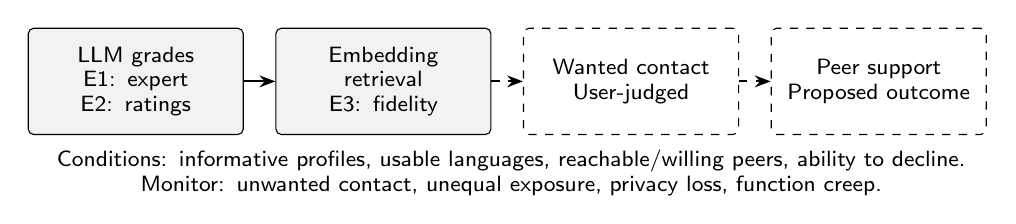
\begin{tikzpicture}[
  box/.style={draw, rounded corners=2pt, align=center,
    text width=2.45cm, minimum height=1.35cm, inner sep=4pt,
    font=\fontsize{8}{9}\selectfont\sffamily},
  link/.style={-{Stealth[length=2mm]}, thick},
  node distance=0.40cm
]
\node[box, fill=black!5] (grades)
  {LLM grades\\E1: expert\\E2: ratings};
\node[box, fill=black!5, right=of grades] (retrieval)
  {Embedding retrieval\\E3: fidelity};
\node[box, dashed, right=of retrieval] (exchange)
  {Wanted contact\\User-judged};
\node[box, dashed, right=of exchange] (support)
  {Peer support\\Proposed outcome};
\draw[link] (grades) -- (retrieval);
\draw[link, dashed] (retrieval) -- (exchange);
\draw[link, dashed] (exchange) -- (support);
\node[align=center, inner sep=0pt, font=\fontsize{8}{9}\selectfont\sffamily, text width=12.1cm,
  below=0.18cm of retrieval.south east, anchor=north, xshift=0.25cm]
  {Conditions: informative profiles, usable languages, reachable/willing peers, ability to decline.\\
   Monitor: unwanted contact, unequal exposure, privacy loss, function creep.};
\end{tikzpicture}
\Description{Medical-LLM grades are assessed against one expert and historical user ratings. An embedding retrieval model is assessed for fidelity to those grades. Dashed links from retrieval to mutually wanted contact and helpful peer support remain untested. Conditions and harms to monitor appear below.}
\caption{Evidence-to-pathway map. Solid links are assessed here (E1--E3);
dashed links are the targets of a consented, beneficiary-informed outcome study.}
\label{fig:change}
\end{figure}


\paragraph{From Ranked Profiles to Wanted Contact.}
Suitable peers must exist, be reachable and wish to engage. The Hit@10 of 0.90 of
our fine-tuned (FT) embedding retrieval model, \model{FT~Arctic+cosine}, means
it retrieves a teacher-score-$\geq4$ peer for about 90\% of evaluated test
queries (Sect.~\ref{sec:fidelity}), against 0.52 for random ordering and 0.72
for the deployed rules.
Contact is also two-sided: reciprocal recommenders score each direction from that person's own
preferences~\cite{pizzato2010recon}, which a single symmetric similarity or expert
score cannot. Contact therefore requires the ability to decline,
informative profiles and usable languages.

\paragraph{Who Might Be Missed or Harmed?}
The rubric's highest grades favor shared diagnoses (Sect.~\ref{sec:profiles}),
potentially disadvantaging undiagnosed members. Demographic matching may
reinforce homophily. The rubric rewards shared conditions at different stages,
which can offer insight but also cause distress.

Better discovery can also increase unwanted exposure, and rankings may
concentrate attention on a few members~\cite{biega2018attention}: on the test
lists, the pairwise MLP scorers give their most-exposed 10\% of candidates 44\% of
top-ten slots, versus 26\% under the deployed rules and 38\% under
\model{FT~Arctic+cosine} (Sect.~\ref{sec:exposure}). Peers pushing lay diagnoses can be unwelcome, and professional or advocacy
accounts may treat a group as serving their own agenda rather than its
members'~\cite{doyle2024support}; the index could also be repurposed for
marketing or recruitment. Responsible deployment requires purpose-limited access,
control over visibility and contact, blocking/reporting, and separation from
medical advice.

A future study should compare mutually accepted contact and helpfulness while monitoring
unwanted contact, exposure and subgroup coverage. The evaluations below address
the earlier step: whether profile judgments provide a useful retrieval signal.

\section{From Profiles to Learned Matchers}
\label{sec:method}
\subsection{Preparing Profiles and Grading Pairs}
\label{sec:profiles}
The dataset contains 3,584 profiles with diagnoses and symptoms coded as
ontology identifiers, demographic fields and free text. The operator pseudonymized them before processing,
and the LLM ran locally. Before transcription, each profile's disease and symptom
identifiers are resolved against the disease ontology, and these entries are
added as context; MedGemma 27B then translates the German JSON profiles into
English and transcribes them into Markdown, which both teacher and students use.

The teacher assesses each unordered, non-self pair:
$3{,}584(3{,}584-1)/2=6{,}420{,}736$ possible judgments. An expert-informed
additive rubric awards up to five points: one if both users live with a rare
disease and seek peer connection; a second for overlapping challenges,
emotional goals or caregiving roles; a third for similar clinical
characteristics such as shared symptoms, affected systems or disease
trajectory; a fourth for experiential and medical complementarity, for example
the same condition at different stages or medically related conditions; and a
fifth only for the same or closely related diagnoses together with goals and
life contexts that promise a mutually beneficial exchange. The prompt also asks
the model to weigh demographics and disease ontologies.

The prompt requests examination, rubric application and justification within
800 words, then a score. Of 6,420,736 pairs, a random 2.0\% were not graded and 2.4\%
fail schema filtering, leaving 6,136,498 valid grades (95.6\%). They concentrate at 1--2 (84\%), with 7.2\% at 4--5, whereas the deployed rules
concentrate near zero (Fig.~\ref{fig:score-and-split}(a)).
Grading all pairs, not a shortlist, avoids preselecting candidates.

\subsection{Learning an Embedding Retrieval Model and a Pairwise MLP Scorer}
To avoid asking the teacher about every pair, the embedding retrieval model embeds a profile $x_u$ as its profile vector
$e_u=f_\theta(x_u)/\|f_\theta(x_u)\|_2$ and scores two profiles with
$s(u,v)=e_u^\top e_v$. Each candidate's profile vector can be reused across queries.

We use Snowflake Arctic Embed M v2.0~\cite{yu2024arcticembed20multilingualretrieval} as the encoder
(\model{Arctic+cosine}). Inputs are truncated to 512 tokens, mean-pooled and $\ell_2$-normalized. Fine-tuning (\model{FT~Arctic+cosine}) uses CoSENT~\cite{huang2024cosent} loss, which penalizes
cosine orderings that contradict the graded labels rather than requiring
a binary positive/negative threshold. Its scale is 20.
Optimization uses AdamW with learning rate $10^{-5}$ and weight decay
$10^{-2}$, for 20 epochs of 264,000 pairs.

The second student, the pairwise MLP scorer, is a multilayer perceptron (MLP) on
concatenated pairs of frozen profile vectors.
It has a 512-unit hidden layer, ReLU and dropout of 0.1, and predicts the teacher's
grade using mean squared error. Training uses Adam, learning rate $10^{-4}$,
weight decay $10^{-5}$, 200 epochs, and up to $10^6$ pairs per epoch.
We train it on pretrained and on fine-tuned profile vectors (\model{Arctic+MLP}, \model{FT~Arctic+MLP}); a linear scorer without the hidden
layer (\model{Arctic+linear}) is an ablation.

Grades are imbalanced, so each training epoch draws pairs with probability
proportional to $1/(K n_y)$, where $n_y$ is the frequency of level $y$ among the
$K=6$ levels; every level then contributes equally. Checkpoints are selected by
full-list validation NDCG (epoch 4 of 20 for the encoder; epochs 54 and 166 of
200 for \model{Arctic+MLP} and \model{FT~Arctic+MLP}). As validation and test
share users, selection may favor the students slightly: the selected epochs exceed
the median epoch's validation NDCG@5 by about 0.01. Validation and test
use all pairs, with their natural grade distribution. Comparators are the deployed rules and
two pretrained embedding retrieval models, \model{Arctic+cosine} and \model{MSMARCO+cosine} (MSMARCO BERT Base Dot
v5,\footnote{\url{https://huggingface.co/sentence-transformers/msmarco-bert-base-dot-v5}}
a Sentence-BERT model~\cite{DBLP:journals/corr/abs-1908-10084} trained on
MS~MARCO~\cite{bajaj2018msmarco}).

\subsection{Separating Training from Evaluation}
Of the 3,584 users, 356 are held out. Validation and test share these users
but not pairs: each split holds 30,153 pairs, and the test split covers 48\% of
the held-out users' possible pairs, 8.4\% of them teacher-high (teacher grade
$\geq4$). Training uses
exactly the 4,977,892 graded pairs among the other 3,228 users; all 1,098,300
cross pairs are excluded from training, and their rated pairs evaluate newcomers
(Sect.~\ref{sec:ratings}; Fig.~\ref{fig:score-and-split}(b)).

\newcommand{\datasetSplitDiagram}{%
  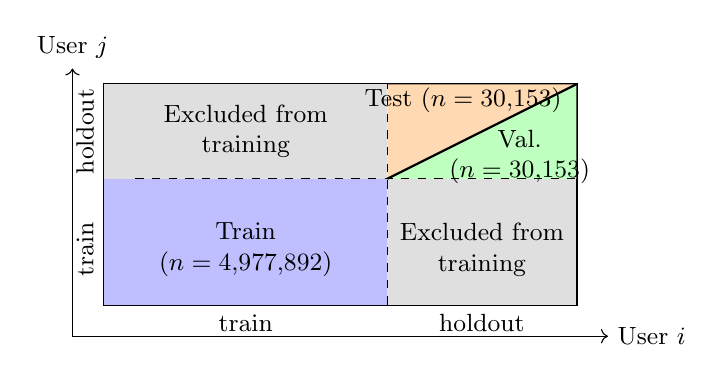
\begin{tikzpicture}[x=0.8cm,y=0.4cm,font=\small]
    \draw[->] (0,0) -- (8.5,0) node[right] {User $i$};
    \draw[->] (0,0) -- (0,8.5) node[above] {User $j$};

    \draw[thick] (0.5,1.0) rectangle (8,8);

    \fill[blue!25] (0.5,1.0) rectangle (5,5);

    \fill[gray!25] (0.5,5) rectangle (5,8);
    \fill[gray!25] (5,1.0) rectangle (8,5);

    \fill[green!25] (5,5) -- (8,5) -- (8,8) -- cycle;
    \fill[orange!30] (5,5) -- (5,8) -- (8,8) -- cycle;

    \draw[dashed] (5,1.0) -- (5,8);
    \draw[dashed] (1.0,5) -- (8,5);
    \draw[thick] (5,5) -- (8,8);

    \node[align=center] at (2.75,2.75) {Train\\$(n=4{,}977{,}892)$};
    \node[align=center] at (2.75,6.5) {Excluded from\\training};
    \node[align=center] at (6.5,2.75) {Excluded from\\training};
    \node[align=center] at (7.1,5.7) {         Val. \\$(n=30{,}153)$};
    \node[align=center] at (6.2,7.5) {Test $(n=30{,}153)$};

    \node[below] at (2.75,1) {train};
    \node[below] at (6.5,1) {holdout};
    \node[rotate=90] at (0.2,2.75) {train};
    \node[rotate=90] at (0.2,6.5) {holdout};
  \end{tikzpicture}%
}

\begin{figure}[!htb]
\centering
\begin{minipage}[b]{0.38\linewidth}
\centering
\resizebox{!}{3.55cm}{\definecolor{sdTeacher}{HTML}{000000}\definecolor{sdGemma}{HTML}{0072B2}\definecolor{sdSmall}{HTML}{009E73}\definecolor{sdRules}{HTML}{CC79A7}%
\begin{tikzpicture}[
  font=\fontsize{8}{9}\selectfont\sffamily,
  tick/.style={font=\fontsize{7}{8}\selectfont\sffamily, inner sep=1.5pt},
  plabel/.style={font=\fontsize{6}{7}\selectfont\sffamily, inner sep=1.2pt},
  curve/.style={line width=0.9pt, line join=round},
  pt/.style={circle, fill, inner sep=0pt, minimum size=2.6pt},
]
\begin{scope}[xshift=0.75cm, yshift=0.6cm, x=0.68cm, y=2.952cm]
  \draw[line width=0.4pt] (0,0) -- (5,0);
  \draw[line width=0.4pt] (0,0) -- (0,1);
  \foreach \x in {0,1,2,3,4,5}
    \draw (\x,0) -- (\x,-0.02) node[tick, below] {\x};
  \foreach \y/\l in {0.2/0.2,0.4/0.4,0.6/0.6,0.8/0.8,1/1}
    \draw (0,\y) -- (-0.06,\y) node[tick, left] {\l};
  \draw[curve, sdTeacher, solid] plot coordinates {(0,0.030697) (1,0.366514) (2,0.475334) (3,0.055908) (4,0.063475) (5,0.008072)};
  \draw[curve, sdGemma, solid] plot coordinates {(0,0.000240) (1,0.098097) (2,0.370895) (3,0.284402) (4,0.219132) (5,0.027233)};
  \draw[curve, sdSmall, solid] plot coordinates {(0,0.398097) (1,0.348228) (2,0.153594) (3,0.043005) (4,0.029642) (5,0.027435)};
  \draw[curve, sdRules, densely dotted] plot coordinates {(0,0.792386) (1,0.144023) (2,0.020425) (3,0.005871) (4,0.000292) (5,0.037004)};
  \foreach \x/\y in {0/0.030697,1/0.366514,2/0.475334,3/0.055908,4/0.063475,5/0.008072} \node[pt, sdTeacher] at (\x,\y) {};
  \foreach \x/\y in {0/0.000240,1/0.098097,2/0.370895,3/0.284402,4/0.219132,5/0.027233} \node[pt, sdGemma] at (\x,\y) {};
  \foreach \x/\y in {0/0.398097,1/0.348228,2/0.153594,3/0.043005,4/0.029642,5/0.027435} \node[pt, sdSmall] at (\x,\y) {};
  \foreach \x/\y in {0/0.792386,1/0.144023,2/0.020425,3/0.005871,4/0.000292,5/0.037004} \node[pt, sdRules] at (\x,\y) {};
  \draw[curve, sdTeacher, solid] (1.6,0.97) -- ++(0.45,0);
  \node[plabel, anchor=west] at (2.15,0.97) {MedGemma 27B teacher};
  \draw[curve, sdGemma, solid] (1.6,0.89) -- ++(0.45,0);
  \node[plabel, anchor=west] at (2.15,0.89) {Gemma 27B};
  \draw[curve, sdSmall, solid] (1.6,0.81) -- ++(0.45,0);
  \node[plabel, anchor=west] at (2.15,0.81) {MedGemma 1.5 4B};
  \draw[curve, sdRules, densely dotted] (1.6,0.73) -- ++(0.45,0);
  \node[plabel, anchor=west] at (2.15,0.73) {Deployed rules};
  \node[anchor=north] at (2.5,-0.142) {Predicted score};
  \node[rotate=90, anchor=south] at (-0.7,0.5) {Fraction of pairs};
\end{scope}
\end{tikzpicture}
}\\[-2pt]
\small (a) Score distributions
\end{minipage}\hfill
\begin{minipage}[b]{0.60\linewidth}
\centering
\resizebox{!}{3.55cm}{\datasetSplitDiagram}\\[-2pt]
\small (b) Pair-matrix split
\end{minipage}
\Description{Left: line plot of the fraction of pairs at each predicted score from 0 to 5. The deployed rules baseline put about 79 percent of pairs at score 0. MedGemma 27B peaks at score 2 (about 48 percent), with about 7 percent at scores 4 and 5; Gemma 27B peaks at score 2 and assigns more scores 3 and 4; MedGemma 1.5 4B declines from about 40 percent at score 0. Right: a user-by-user pair matrix split into training users and holdout users. Train--train pairs form the training set of 4,977,892 pairs, train--holdout pairs are excluded from training, and the holdout--holdout block is divided into validation and test pairs of 30,153 each.}
\caption{(a) Score distributions of the deployed rules (all pairs they score)
and of the LLM graders: the rules concentrate near zero, while the LLMs assign
more intermediate and high grades. (b) Pairs of a training and a held-out user are excluded from training (their
rated pairs evaluate newcomers); the holdout--holdout region is partitioned into
validation and test pairs.}
\label{fig:score-and-split}
\end{figure}

\section{Three Views of the Evidence}
\label{sec:findings}
\subsection{E1: Does the Teacher Agree with an Expert?}
One HCP saw parsed profiles, but not the teacher's
labels, and scored from 0 to 5 whether each pair might be interested in
interacting. Like stratified validation of LLM relevance labels~\cite{merlo2026stratified}, we
stratify by the teacher's score: sampling eleven pairs at each level yields 66
judgments and covers the full score range. All 66
pairs and their 93 users come from the test split, so no student saw them in
training.
Because these are pairs rather than complete candidate lists, we use
Spearman correlation.

The teacher agrees more closely with this HCP than the deployed rules do:
0.78 versus 0.53 (Table~\ref{tab:expert-ecir}), supporting its use as supervision.
The paired difference of 0.25 has a 95\% interval of 0.07--0.47 and stays
between 0.18 and 0.28 when any one of the 93 users is left out. Distillation
carries this agreement over to held-out users: students trained on teacher
grades reach 0.80--0.84, whereas \model{Arctic+cosine} reaches 0.51
(fine-tuning it, \model{FT~Arctic+cosine}, adds 0.31, interval 0.11--0.52). The students' edge over the
teacher (0.02--0.06) is within sampling error; their continuous scores also
break the ties among the teacher's six grades.

\begin{table}[!htb]
\caption{Spearman agreement with the HCP on 66 teacher-stratified test pairs.
Intervals: 10,000 bootstrap resamples of pairs within teacher-grade strata.
FT: fine-tuned.}
\label{tab:expert-ecir}
\centering
\setlength{\tabcolsep}{5pt}
\begin{tabular}{lrr}
\toprule
Scorer & $\rho$ & 95\% CI \\
\midrule
Deployed rules & 0.53 & 0.33--0.70 \\
MedGemma 27B teacher & 0.78 & 0.67--0.87 \\
\model{Arctic+cosine (pretrained)} & 0.51 & 0.30--0.70 \\
\model{Arctic+MLP} & 0.84 & 0.75--0.91 \\
\model{FT Arctic+cosine} & 0.82 & 0.72--0.89 \\
\model{FT Arctic+MLP} & 0.80 & 0.69--0.88 \\
\bottomrule
\end{tabular}
\end{table}

The high grades illustrate a trade-off.
Of eleven HCP-high pairs (score $\geq4$), nine are teacher-high and one is
rules-high. The deployed rules miss ten at this threshold.
Conversely, only nine of the 22 teacher-high pairs are HCP-high: the teacher
grades more permissively than the HCP.

\subsection{E2: Do the Grades Align with Users' Historical Ratings?}
\label{sec:ratings}
Members also rate suggested peers: 15,356 feedback records cover 14,889 pairs,
13,697 of them with a valid teacher grade. For users with at least two such
candidates, we rank them and compare their order with feedback using normalized
discounted cumulative gain (NDCG), which emphasizes the top of the ranking.

On all rated pairs, MedGemma 27B exceeds the deployed rules at each cutoff
(Table~\ref{tab:feedback}, upper block; NDCG@5 difference 0.06, 95\% interval
0.05--0.07 over users).
Rated lists are short (median six candidates for 1,915 users), so random order
already reaches NDCG@5 0.56; both scorers clear it. We chose MedGemma 27B
without consulting the ratings, so E2 is an independent check of the teacher;
exploratory Gemma 3 27B~\cite{gemmateam2025gemma3} and MedGemma 1.5
4B~\cite{sellergren2026medgemma15} runs
on a uniformly sampled 1\% of pairs appear only in
Fig.~\ref{fig:score-and-split}(a).

Students can only be checked on ratings of users they never saw. We therefore treat
the held-out users as newcomers: each ranks the training users it rated or was
rated by. These newcomer--training pairs were excluded from training (2,930 rated
pairs from 201 newcomers; Table~\ref{tab:feedback}, lower block). \model{FT~Arctic+cosine} exceeds the rules by
0.09 NDCG@5 (95\% interval 0.06--0.12), and fine-tuning adds 0.07 (0.04--0.09)
over \model{Arctic+cosine}. It also edges the teacher (0.03, 0.01--0.05),
possibly because the teacher's six grades leave many ties; checkpoint selection
may account for about 0.01 of this.

Figure~\ref{fig:feedback} groups 13,697 pairs by teacher score, with
feedback averaged within each pair. Higher score groups tend to have higher
feedback, but the pattern is not monotonic: the 134 score-zero pairs have
relatively high feedback. Inspection linked this exception to sparse profiles
and possible offline acquaintance.

\begin{figure}[!tb]
\centering
\begin{minipage}[t]{0.53\textwidth}
\vspace{0pt}
\captionof{table}[Ranking agreement with historical user feedback]{\raggedright
Ranking agreement with historical user feedback: NDCG over
each user's rated candidates; rows within a block rank the same lists. Newcomers:
held-out users ranking the training users they rated or were rated by.
Random order is the exact expectation. FT: fine-tuned. Differences in the text
are computed before rounding.}
\label{tab:feedback}
\smallskip
\centering\footnotesize
\setlength{\tabcolsep}{2.5pt}
\renewcommand{\arraystretch}{1.05}
\begin{tabular}{lrrr}
\toprule
& \multicolumn{3}{c}{NDCG} \\
Scorer & @5 & @10 & @all \\
\midrule
\multicolumn{4}{l}{\textit{All users (1,915)}} \\
Random order & 0.56 & 0.62 & 0.69 \\
Deployed rules & 0.66 & 0.70 & 0.75 \\
MedGemma 27B teacher & \textbf{0.71} & \textbf{0.75} & \textbf{0.79} \\
\addlinespace[2pt]
\multicolumn{4}{l}{\textit{Newcomers (201)}} \\
Random order & 0.58 & 0.63 & 0.69 \\
Deployed rules & 0.69 & 0.72 & 0.76 \\

\shortstack[l]{MedGemma 27B\\teacher} & 0.75 & 0.77 & 0.80 \\
\model{MSMARCO+cosine} & 0.71 & 0.74 & 0.78 \\
\model{Arctic+cosine} & 0.71 & 0.75 & 0.78 \\
\model{Arctic+MLP} & 0.72 & 0.75 & 0.78 \\
\model{FT Arctic+cosine} & \textbf{0.77} & \textbf{0.80} & \textbf{0.82} \\
\model{FT Arctic+MLP} & 0.74 & 0.77 & 0.80 \\
\bottomrule
\end{tabular}
\end{minipage}\hfill
\begin{minipage}[t]{0.44\textwidth}
\vspace{0pt}
\centering
\resizebox{\linewidth}{!}{\begin{tikzpicture}[x=0.007cm,y=0.0122cm,
  font=\fontsize{8}{9}\selectfont\sffamily]
\useasboundingbox (-45,70) rectangle (945,920);
\begin{scope}
  \clip (83,130) rectangle (935,906);
  \node[anchor=south west,inner sep=0pt] at (0,0)
    {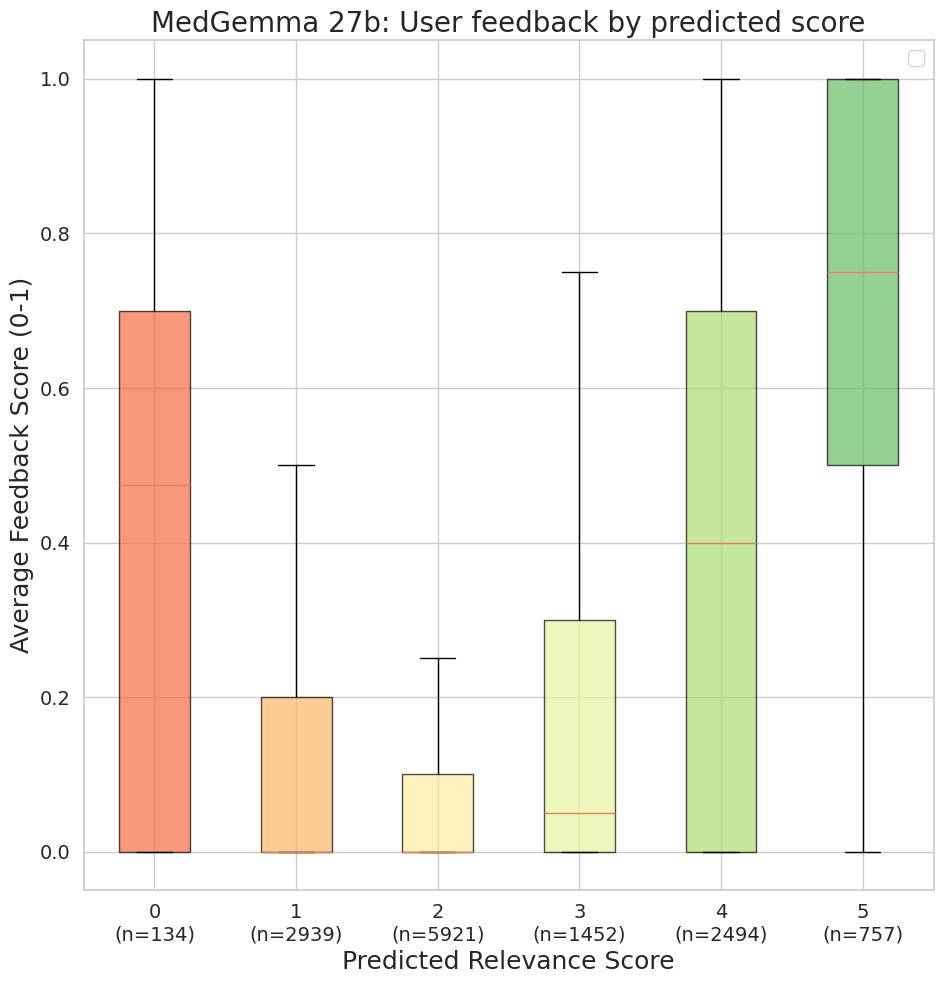
\includegraphics[width=6.601cm,height=12.005cm]{figures/medgemma-vs-feedbackavg.png}};
\end{scope}
\foreach \value in {0,0.2,0.4,0.6,0.8,1} {
  \pgfmathsetmacro{\tickY}{131+774*\value}
  \node[anchor=east,inner sep=2pt] at (83,\tickY) {\value};
}
\foreach \grade in {0,...,5} {
  \pgfmathsetmacro{\tickX}{84+(\grade+0.5)*850/6}
  \node[anchor=north,inner sep=3pt] at (\tickX,130) {\grade};
}
\node[anchor=north,inner sep=0pt] at (509,99) {Teacher grade (MedGemma 27B)};
\node[rotate=90,inner sep=0pt] at (-15,518) {Mean user feedback};
\end{tikzpicture}
}
\Description{Original box plot of average user feedback per pair by MedGemma score 0 to 5. Bin counts are 134, 2939, 5921, 1452, 2494 and 757, totaling 13697 pairs. Feedback is generally higher in the upper score groups, with a small high-feedback score-zero group.}
\setlength{\abovecaptionskip}{2pt}%
\captionof{figure}[Mean user feedback per pair by teacher grade]{\raggedright
Mean user feedback per pair by teacher grade. Grades 0--5
contain 134, 2,939, 5,921, 1,452, 2,494 and 757 pairs, respectively.}
\label{fig:feedback}
\end{minipage}
\end{figure}

\subsection{E3: Can a Smaller Model Learn the Teacher's Ordering?}
\label{sec:fidelity}
Does this signal survive distillation? On the teacher-labeled test split (356
users, a median of 169 candidates per query), NDCG measures ordering by teacher
grade, while Precision (P) and Hit Rate (Hit) use
grade $\geq4$.

Table~\ref{tab:fidelity-ecir} shows that learning from these grades improves
top-ranked agreement. Fine-tuning \model{Arctic+cosine} into \model{FT~Arctic+cosine} raises NDCG@5 from
0.64 to 0.77, against 0.43 for random order, and improves NDCG@10 for 319 of
the 356 test users (mean $+0.13$). \model{Arctic+MLP} already reaches 0.74; without its hidden layer,
\model{Arctic+linear} falls to 0.57, below \model{Arctic+cosine}, because it ranks
every query's candidates alike (Sect.~\ref{sec:exposure}). Holding the scorer type fixed, the fine-tuned encoder's
NDCG@5 is about 0.13 higher under cosine and 0.02 higher under the MLP.

\begin{table}[!tb]
\caption{Teacher-label fidelity on the test split: how well each model
reproduces the teacher's ranking of candidates for users excluded from
training, not how the users themselves would rank them. NDCG@5 is the primary
top-ranked metric; P and Hit use teacher score $\geq4$. Random order is the
exact expectation. FT means fine-tuned.}
\label{tab:fidelity-ecir}
\centering
\footnotesize
\setlength{\tabcolsep}{3pt}
\renewcommand{\arraystretch}{1.05}
\begin{tabular}{lrrrrrrr}
\toprule
& \multicolumn{3}{c}{NDCG} & \multicolumn{2}{c}{P} & \multicolumn{2}{c}{Hit} \\
Model & @5 & @10 & @all & @5 & @10 & @5 & @10 \\
\midrule
Random order (expected) & 0.43 & 0.46 & 0.86 & 0.09 & 0.09 & 0.34 & 0.52 \\
\addlinespace[2pt]
\multicolumn{8}{l}{\textbf{Pretrained embedder baselines (cosine)}} \\
\model{MSMARCO BERT Base Dot v5} & 0.60 & 0.62 & 0.90 & 0.30 & 0.26 & 0.67 & 0.74 \\
\model{Arctic Embed M v2.0} & 0.64 & 0.65 & 0.91 & 0.35 & 0.31 & 0.67 & 0.75 \\
\addlinespace[2pt]
\multicolumn{8}{l}{\textbf{Existing task baseline}} \\
Deployed rules & 0.58 & 0.59 & 0.89 & 0.26 & 0.23 & 0.60 & 0.72 \\
\addlinespace[2pt]
\multicolumn{8}{l}{\textbf{Our models}} \\
\model{Arctic+linear} & 0.57 & 0.60 & 0.90 & 0.22 & 0.20 & 0.50 & 0.64 \\
\model{Arctic+MLP} & 0.74 & 0.76 & \textbf{0.94} & 0.48 & 0.43 & 0.81 & 0.88 \\
\model{FT Arctic+cosine} & \textbf{0.77} & \textbf{0.78} & \textbf{0.94} & \textbf{0.54} & \textbf{0.48} & \textbf{0.84} & 0.90 \\
\model{FT Arctic+MLP} & 0.76 & \textbf{0.78} & \textbf{0.94} & 0.51 & 0.46 & \textbf{0.84} & \textbf{0.91} \\
\bottomrule
\end{tabular}
\end{table}

Full-list NDCG hardly separates scorers, since random order already reaches
0.86. The deployed rules beat random order (NDCG@5 0.58 versus 0.43) but trail
the pretrained embedding retrieval models.
\model{FT~Arctic+cosine} matches \model{FT~Arctic+MLP} (0.77 versus 0.76 NDCG@5)
while reusing one vector per profile. E3 measures fidelity to the
teacher, which by itself is no evidence of
quality~\cite{dietz2025judges,soboroff2025judgments}; E1 and E2 anchor the
teacher to human judgments.

\subsection{Who Gets Shown? Exposure on the Test Lists}
\label{sec:exposure}
Exposure asks who gets suggested, not whether a suggestion is good. We measure
it on the test lists of Table~\ref{tab:fidelity-ecir}: each of the 356 users
excluded from training acts as a query over a median of 169 candidates
(144--196), and every scorer fills a top ten, giving 3,560 suggestion slots. A
user's exposure is the number of slots they receive, averaging ties. It needs no
labels and says nothing about individual match quality: it shows how evenly a
scorer spreads its suggestions (Table~\ref{tab:exposure}, Fig.~\ref{fig:exposure}).
The Gini coefficient is 0 if every user is suggested equally often and
approaches 1 if a few users take all slots; Top 10\% is the share of slots held
by the most-suggested tenth of users (0.10 under equality); Never counts users
in nobody's top ten. Two diagnostics explain the differences: Overlap is the
share of a scorer's top ten that the deployed rules would also show, and the
profile $R^2$, defined next, measures how much a scorer's ranking depends on who
the candidate is, regardless of who is searching.

Following baseline estimates in recommendation~\cite{koren2008factorization}
and the social relations model for dyads~\cite{kenny1984social}, we fit each
scorer's test scores as $s(u,v)\approx\mu+a_u+a_v$. Each member has one effect
$a_u$, how highly the scorer rates $u$ with anyone, and the effects sum to zero.
We minimize the squared error over all observed test pairs by alternating
updates, setting each $a_u$ to the mean residual of $u$'s pairs until the effects
converge. The profile $R^2=1-\sum(s-\hat{s})^2/\sum(s-\bar{s})^2$ is the share of
score variance that this fit explains. Near 0, scores depend on who is paired
with whom, so every member receives a different ranking; near 1, a candidate
scores almost the same for every query, so all members see the same people
first. Order-dependent MLP scores are approximated by effects that are the same in both roles.

\begin{table}[!tb]
\caption{Top-ten exposure on the test lists of Table~\ref{tab:fidelity-ecir} (356 users,
median 169 candidates): how evenly each scorer spreads its suggestions across
users. The exposure columns use no labels and do not measure match quality;
NDCG@5 repeats Table~\ref{tab:fidelity-ecir} and measures agreement with the LLM teacher's
grades, not the HCP's. Columns are defined in Sect.~\ref{sec:exposure}; ties are
averaged and random shows expected exposure. Bold marks the best scorer (highest
NDCG, least concentration). FT means fine-tuned.}
\label{tab:exposure}
\centering
\footnotesize
\setlength{\tabcolsep}{3pt}
\renewcommand{\arraystretch}{1.05}
\begin{tabular}{lrrrrrr}
\toprule
& NDCG & \multicolumn{3}{c}{Top-ten exposure} & \multicolumn{2}{c}{Diagnostics} \\
Model & @5 & Gini & Top 10\% & Never & Overlap & $R^2$ \\
\midrule
Random order (expected) & -- & 0.03 & 0.11 & 0 & 0.06 & -- \\
Teacher-grade order & -- & 0.41 & 0.27 & 0 & 0.15 & 0.30 \\
\addlinespace[2pt]
\multicolumn{7}{l}{\textbf{Pretrained embedder baselines (cosine)}} \\
\model{MSMARCO BERT Base Dot v5} & 0.60 & 0.48 & 0.33 & 14 & 0.14 & 0.31 \\
\model{Arctic Embed M v2.0} & 0.64 & \textbf{0.42} & 0.27 & 12 & 0.16 & 0.28 \\
\addlinespace[2pt]
\multicolumn{7}{l}{\textbf{Existing task baseline}} \\
Deployed rules & 0.58 & 0.43 & \textbf{0.26} & \textbf{8} & -- & 0.26 \\
\addlinespace[2pt]
\multicolumn{7}{l}{\textbf{Our models}} \\
\model{Arctic+linear} & 0.57 & 0.91 & 0.91 & 282 & 0.10 & 0.95 \\
\model{Arctic+MLP} & 0.74 & 0.65 & 0.44 & 82 & 0.17 & 0.60 \\
\model{FT Arctic+cosine} & \textbf{0.77} & 0.53 & 0.38 & 21 & 0.19 & 0.63 \\
\model{FT Arctic+MLP} & 0.76 & 0.63 & 0.44 & 67 & 0.17 & 0.56 \\
\bottomrule
\end{tabular}
\end{table}

\begin{figure}[!tb]
\centering
\definecolor{exRandom}{HTML}{777777}\definecolor{exTeacher}{HTML}{000000}\definecolor{exRules}{HTML}{CC79A7}\definecolor{exMsmarco}{HTML}{999999}\definecolor{exArctic}{HTML}{0072B2}\definecolor{exLinear}{HTML}{000000}\definecolor{exMLP}{HTML}{D55E00}\definecolor{exFT}{HTML}{009E73}\definecolor{exFTMLP}{HTML}{E69F00}%
\begin{tikzpicture}[
  font=\fontsize{8}{9}\selectfont\sffamily,
  tick/.style={font=\fontsize{7}{8}\selectfont\sffamily, inner sep=1.5pt},
  plabel/.style={font=\fontsize{6}{7}\selectfont\sffamily, inner sep=1.2pt},
  curve/.style={line width=0.9pt, line join=round},
  title/.style={anchor=south west, inner sep=0pt,
    font=\fontsize{8}{9}\selectfont\sffamily\bfseries},
]
\begin{scope}[xshift=0.95cm, yshift=0.75cm, x=4.2cm, y=2.952cm]
  \draw[line width=0.4pt] (0,0) -- (1,0);
  \draw[line width=0.4pt] (0,0) -- (0,1);
  \foreach \x in {0,0.2,0.4,0.6,0.8,1}
    \draw (\x,0) -- (\x,-0.02) node[tick, below] {\x};
  \foreach \y in {0.2,0.4,0.6,0.8,1}
    \draw (0,\y) -- (-0.012,\y) node[tick, left] {\y};
  \draw[curve, exRandom, dashed] plot coordinates {(0,0.0000) (0.1,0.1094) (0.2,0.2150) (0.3,0.3185) (0.4,0.4205) (0.5,0.5212) (0.6,0.6206) (0.7,0.7185) (0.8,0.8151) (0.9,0.9092) (1,1.0000)};
  \draw[curve, exTeacher, densely dashdotted] plot coordinates {(0,-0.0000) (0.1,0.2683) (0.2,0.4408) (0.3,0.5771) (0.4,0.6899) (0.5,0.7841) (0.6,0.8627) (0.7,0.9203) (0.8,0.9610) (0.9,0.9878) (1,1.0000)};
  \draw[curve, exRules, densely dotted] plot coordinates {(0,0.0000) (0.1,0.2608) (0.2,0.4448) (0.3,0.5936) (0.4,0.7154) (0.5,0.8132) (0.6,0.8871) (0.7,0.9379) (0.8,0.9722) (0.9,0.9929) (1,1.0000)};
  \draw[curve, exMLP, solid] plot coordinates {(0,0.0000) (0.1,0.4329) (0.2,0.6556) (0.3,0.7966) (0.4,0.8794) (0.5,0.9379) (0.6,0.9751) (0.7,0.9930) (0.8,1.0000) (0.9,1.0000) (1,1.0000)};
  \draw[curve, exFT, solid] plot coordinates {(0,0.0000) (0.1,0.3767) (0.2,0.5615) (0.3,0.6848) (0.4,0.7835) (0.5,0.8570) (0.6,0.9132) (0.7,0.9549) (0.8,0.9822) (0.9,0.9959) (1,1.0000)};
  \draw[curve, exFTMLP, solid] plot coordinates {(0,0.0000) (0.1,0.4351) (0.2,0.6568) (0.3,0.7834) (0.4,0.8662) (0.5,0.9256) (0.6,0.9631) (0.7,0.9855) (0.8,0.9988) (0.9,1.0000) (1,1.0000)};
  \draw[curve, exFTMLP, solid] (0.46,0.41) -- ++(0.09,0);
  \node[plabel, anchor=west] at (0.57,0.41) {\model{FT Arctic+MLP}};
  \draw[curve, exFT, solid] (0.46,0.33) -- ++(0.09,0);
  \node[plabel, anchor=west] at (0.57,0.33) {\model{FT Arctic+cosine}};
  \draw[curve, exMLP, solid] (0.46,0.25) -- ++(0.09,0);
  \node[plabel, anchor=west] at (0.57,0.25) {\model{Arctic+MLP}};
  \draw[curve, exRules, densely dotted] (0.46,0.17) -- ++(0.09,0);
  \node[plabel, anchor=west] at (0.57,0.17) {Deployed rules};
  \draw[curve, exTeacher, densely dashdotted] (0.46,0.09) -- ++(0.09,0);
  \node[plabel, anchor=west] at (0.57,0.09) {Teacher-grade order};
  \node[plabel, rotate=35, anchor=north, text=exRandom] at (0.74,0.73) {random};
  \node[anchor=north] at (0.5,-0.142) {Share of candidates, most exposed first};
  \node[rotate=90, anchor=south] at (-0.137,0.5) {Share of top-ten slots};
  \node[title] at (0,1.049) {(a) Concentration of top-ten exposure};
\end{scope}
\begin{scope}[xshift=5.0cm, yshift=-1.874cm, x=6.0cm, y=6.56cm]
  \draw[line width=0.4pt] (0.35,0.40) -- (1,0.40);
  \draw[line width=0.4pt] (0.35,0.40) -- (0.35,0.85);
  \foreach \x in {0.4,0.6,0.8,1}
    \draw (\x,0.40) -- (\x,0.391) node[tick, below] {\x};
  \foreach \y in {0.4,0.5,0.6,0.7,0.8}
    \draw (0.35,\y) -- (0.345,\y) node[tick, left] {\y};
  \fill[exMsmarco] (0.4849,0.6041) circle (1.6pt);
  \node[plabel, anchor=west, xshift=3pt, yshift=0pt] at (0.4849,0.6041) {\model{MSMARCO+cosine}};
  \fill[exArctic] (0.4200,0.6368) circle (1.6pt);
  \node[plabel, anchor=south west, xshift=1pt, yshift=1pt] at (0.4200,0.6368) {\model{Arctic+cosine}};
  \fill[exRules] (0.4290,0.5804) circle (1.6pt);
  \node[plabel, anchor=north west, xshift=1pt, yshift=-2pt] at (0.4290,0.5804) {Deployed rules};
  \fill[exLinear] (0.9104,0.5726) circle (1.6pt);
  \draw[line width=0.3pt, black!60] (0.9104,0.5726) -- (0.86,0.494);
  \node[plabel, anchor=north] at (0.86,0.49) {\model{Arctic+linear}};
  \fill[exMLP] (0.6462,0.7362) circle (1.6pt);
  \node[plabel, anchor=north west, xshift=2pt, yshift=-1pt] at (0.6462,0.7362) {\model{Arctic+MLP}};
  \fill[exFT] (0.5321,0.7652) circle (1.6pt);
  \node[plabel, anchor=south, xshift=14pt, yshift=4pt] at (0.5321,0.7652) {\model{FT Arctic+cosine}};
  \fill[exFTMLP] (0.6347,0.7599) circle (1.6pt);
  \node[plabel, anchor=west, xshift=3pt, yshift=0pt] at (0.6347,0.7599) {\model{FT Arctic+MLP}};
  \node[anchor=north] at (0.675,0.336) {Exposure Gini};
  \node[rotate=90, anchor=south] at (0.27,0.625) {NDCG@5 (teacher)};
  \node[title] at (0.35,0.872) {(b) Fidelity versus concentration};
\end{scope}
\end{tikzpicture}
\Description{Two panels for the 356 test users. Left: share of top-ten slots held by the most-exposed share of candidates. Random expected exposure follows the diagonal; ordering by the teacher's grades and the deployed rules concentrate least, the fine-tuned cosine retriever more, and the two MLP students most. Right: scatter of teacher NDCG@5 against exposure Gini. The fine-tuned cosine retriever has the highest NDCG@5 with a Gini near 0.53; the MLP students reach similar NDCG@5 with Gini near 0.64; the linear scorer on concatenated embeddings has low NDCG@5 and a Gini of 0.91; the deployed rules and pretrained cosine models have NDCG@5 between 0.58 and 0.64 and Gini between 0.42 and 0.49.}

\caption{Exposure on the test lists (356 users). (a) Share of top-ten slots held by the
most-exposed candidates (deciles; ties averaged, random expected); pretrained
\model{Arctic+cosine} lies on the rules' curve. (b) Teacher NDCG@5
(Table~\ref{tab:fidelity-ecir}) against exposure Gini for each scorer.}
\label{fig:exposure}
\end{figure}


Fidelity and concentration do not rise together (Fig.~\ref{fig:exposure}(b)).
Ordering by the teacher's own grades spreads exposure as evenly as the deployed rules
(Gini 0.41 versus 0.43), so the students' concentration does not come from their
labels. \model{FT~Arctic+cosine} is the most faithful student and
concentrates exposure less than the pairwise MLP scorers (Gini 0.53 versus 0.63--0.65): the MLP scorers never show
67--82 of the 356 candidates, \model{FT~Arctic+cosine} 21 and the rules 8.

\model{Arctic+linear} shows the mechanism in its extreme form. Its score is a
weighted sum of the two profile vectors, so for a given query only the candidate's
part of the sum varies: every query ranks its candidates in nearly the same order,
and the same few candidates fill most top-ten slots (Gini 0.91; 282 of 356
candidates never shown). More generally, concentration
rises with the share of score variance that per-profile effects explain ($R^2$
from 0.26 for the rules to 0.95; Spearman 0.86 across the seven
scorers of Table~\ref{tab:exposure}). The teacher's grades have an $R^2$ of only 0.30, so
the students amplify per-profile effects beyond their labels (0.56--0.63).
Candidates that appear in the top ranks of many queries are known as hubs in
high-dimensional data~\cite{radovanovic2010hubs}; here they
emerge through training on the teacher's grades.
Every scorer shares at most 19\% of its top ten with the deployed rules, so
replacing them would change most suggestions that members see.

\section{Implications for Deployment and Evaluation}
\paragraph{Serving Workload.}
Table~\ref{tab:serving} breaks serving into stages. Every path starts with one LLM
transcription per profile. The teacher then needs one LLM generation per pair;
the students need one encoding per profile and one vector operation per pair,
about \textbf{{\boldmath$6\cdot10^{10}$} times fewer} operations per pair. A new member is thus ranked
against the other 3,583 in 8\,ms after a 6.4\,s transcription, instead of 1.7\,h,
and grading all 6.4 million pairs takes about 125 GPU-days, against 1.6\,h of
transcription and 10\,s of encoding. \model{FT~Arctic+cosine} matches the fidelity of \model{FT~Arctic+MLP}
(Table~\ref{tab:fidelity-ecir}), so serving needs a 1.2\,GB encoder and 11\,MB of
profile vectors; only transcription needs the 27B model, once per profile. Teacher labels,
needed only for training, are the main cost.

\begin{table}[!tb]
\caption{Serving cost per stage on one NVIDIA A100 (80\,GB). Teacher and students
start from one transcription per profile. Times are measured: single requests for
transcribing and encoding a new member, batched runs otherwise. FLOPs are
estimated as $2\times$parameters$\times$tokens for the LLM and the encoder (mean tokens per
request; the encoder reads one Markdown profile) and counted exactly for the scoring heads; memory is that of the
weights or of the profile vectors, which have no parameters (for the MLP, 3\,MB of weights and 15\,MB of first-layer
products precomputed per profile in place of its vectors, so that a pair needs only a 512-dimensional
addition and dot product). LLM FLOPs count input and output tokens alike,
but output tokens are generated one at a time, so measured times are the better
guide to cost.}
\label{tab:serving}
\centering
\footnotesize
\setlength{\tabcolsep}{3pt}
\renewcommand{\arraystretch}{1.05}
\resizebox{\linewidth}{!}{%
\begin{tabular}{llrlcrrrrr}
\toprule
& & & & & & \multicolumn{2}{c}{New member} & \multicolumn{2}{c}{All pairs} \\
\cmidrule(lr){7-8}\cmidrule(lr){9-10}
Stage & Model (memory) & Params & Unit & Tokens in/out & FLOPs/unit & units & time & units & time \\
\midrule
Transcription & MedGemma 27B (54\,GB) & 27\,B & profile & 3,912/212 & $2.2\cdot10^{14}$ & 1 & 6.4\,s & 3,584 & 1.6\,h \\
\addlinespace[2pt]
\multicolumn{10}{l}{\textit{Teacher}} \\
Grading & MedGemma 27B (54\,GB) & 27\,B & pair & 959/824 & $9.6\cdot10^{13}$ & 3,583 & 1.7\,h & 6.4\,M & 125\,d \\
\addlinespace[2pt]
\multicolumn{10}{l}{\textit{Students}} \\
Encoding & Encoder (1.2\,GB) & 305\,M & profile & 212/-- & $4.8\cdot10^{10}$ & 1 & 8\,ms & 3,584 & 10\,s \\
Cosine scoring & Profile vectors (11\,MB) & -- & pair & -- & $1.5\cdot10^{3}$ & 3,583 & 0.09\,ms & 6.4\,M & 0.5\,ms \\
MLP scoring & MLP (18\,MB) & 0.79\,M & pair & -- & $2.0\cdot10^{3}$ & 3,583 & 0.15\,ms & 6.4\,M & 0.09\,s \\
\bottomrule
\end{tabular}}
\end{table}

\paragraph{Scope and Next Steps.}
\label{sec:limitations}
One HCP judged 66 teacher-stratified test pairs; a second blinded annotator
would test the reliability of these judgments.
Feedback covers only candidates the deployed rules had shown, so E2 compares scorers
within those lists; newcomers' lists are short (median five rated candidates). The rubric is not yet beneficiary-validated. The exposure audit covers the 356 test users rather
than the whole platform.
Diagnosis and completeness breakdowns, repeated runs and a beneficiary study
of the contact-to-support pathway complete the agenda.

\paragraph{Ethics and Data Governance.}
Scores are peer-discovery suggestions, not medical advice.
The algorithms were developed for the platform's matching service. The
platform was developed with a university hospital's data protection officer
and in consultation with the local ethics committee; under the committee's
statutes no formal vote was required, as the work is neither a clinical trial of a
medicinal product nor a clinical investigation of a medical
device~\cite{fendrich2026development}.
The operator pseudonymized all profiles before processing; we ran all LLM
inference locally on academic infrastructure in Germany. Because even
pseudonymized health attributes and embeddings can enable re-identification or
text recovery~\cite{elemam2011reidentification,morris2023embeddings}, profiles,
embeddings and labels will not be released.

\section{Conclusion}
Where interaction data are too sparse, a medical LLM can supply the relevance
judgments that peer retrieval needs. In this rare-disease community, MedGemma
27B agrees more closely than the deployed rules with an expert and with
historical ratings. Its grades teach the embedding retrieval model \model{FT~Arctic+cosine}, which raises fidelity
from 0.64 to 0.77 NDCG@5 for users excluded from training. This model ranks
these users' rated peers better than the deployed rules (0.77 versus 0.69
NDCG@5) and agrees with the expert as closely as the teacher. The pipeline is
also efficient end to end: on one A100 GPU, a new member is transcribed and
ranked against the other 3,583 in 6.4\,s instead of 1.7\,h with the teacher,
and all 3,584 profiles in 1.6\,h instead of 125 GPU-days. \model{FT~Arctic+cosine}
concentrates exposure less than the pairwise MLP scorers, but every learned model would replace most current suggestions, which deployment should
monitor. Next comes a consented study of mutually wanted, helpful contact and
its harms.

\begin{credits}
\subsubsection{Use of Generative AI.}
Generative models are part of the method: MedGemma 27B transcribes and
translates profiles and produces the teacher grades (Sect.~\ref{sec:profiles}).
Separately, OpenAI Codex and Anthropic Claude Code assisted with drafting text,
editing, figure and analysis code, and review. The authors reviewed all
generated text, code and reported numbers.
\subsubsection{\discintname}
The authors declare no financial competing interests. They developed the
reported algorithms for a non-profit platform.
\end{credits}

\clearpage
\bibliographystyle{splncs04}
\bibliography{references}
\end{document}
